\chapter{Gaiting and Gait-Stability Control}
\label{ch::gait_control}



	\section{Overview}

		Legged robotic systems have long employed motion controllers based on limit cycle oscillators and, more recently, Central Pattern Generators (CPGs)  for the purpose of generating bio-mimetic gaits \cite{Matsuoka1985,Collins1993,Endo2004,Righetti2006,Ijspeert2008,Matos2010,Ajallooeian2013,Park2014,Fukuoka2015}. Since these motion control methods are open-loop motion planners (\IE not inherently formulated to incorporate feedback) they do not perform any active syste stabilization on their own accord. As a result, implementations involving these  locomotion methods often require auxiliary control mechanisms which provide gait stability. Fixed point methods, which include considerations of the system's zero-moment point (ZMP) and center of gravity (COG), are utilized in the design of stable oscillator driven gaits. These methods are summarized in \cite{Wieber2015}. %add ZMP references%

		Developments in CPG-based gait controllers have led to the incorporation of ``reflexive" feedback mechanisms aimed at correcting foot-placement during gaiting on uneven terrain or various surfaces. One such approach involves active compliance to each leg by directly modifying CPG oscillators units through feedback-driven modulations. In \cite{Fukuoka2003} and \cite{Endo2004}, a CPG for each leg is modified by a neural oscillator with one tuning parameter. 

		This chapter will detail a similar, reflex-adaptive CPG gait generation method which utilizes IMU feedback to modify CPG limit-cycle parameters. Additionally, this section will present related motion-control methods implemented on the BlueFoot platform which aid in gait stabilization, including a virtual force-based foot placement planner and a ZMP-based body placement controller; as well as a nuero-control technique used to level BlueFoot's trunk.




	\section{Central Pattern Generator (CPG) Based Gaiting}

		A central pattern generator (CPG), which includes a reflexive mechanism using sensory feedback, is utilized as the core of the robot's gait generation algorithm. CPGs are a form of neural oscillator network which mimic biological mechanisms for repetitive motor tasks \cite{Ijspeert2008}, \cite{Collins1993}. CPGs commonly consist of a network of multi-state unit-oscillators. These unit-oscillators are coupled such that the motion of one oscillator drives or attenuates the motion of other oscillators it is connected to, creating phase-locked limit cycles.

		In this context, the limit-cycles generated with a CPG will be utilized to drive a quadruped  walking gait by mapping oscillator outputs to foot position controls. CPGs are widely used in this way as they provide a compact method for prescribing rhythmic gaits with variable stepping sequences 
		\cite{
			Righetti2006,
	 		Castro2008,
			Li2014
		}. 
		CPG-driven gait controllers are convenient as they allow for continuous transitioning between gaiting patterns through the modification of oscillator coupling. Reflexes are built into the oscillators which use IMU measurements to modulate the CPGs unit oscillators, as will be outlined later in this section.

		The CPG implemented on BlueFoot consists of four modified two-state ($y_{1,i},y_{2,i}$) Hopf Oscillators connected through a coupling matrix $K$.  The oscilator output vector, $y_{2,i}$, parameterize the trajectories of each \Ith foot. The resulting reflexive CPG system is described by
		\begin{eqnarray}
			\dot{y}_{1} &=& A_{1}\wrap{ \Psi_{M} M - \Gamma}{y}_{1} + \Psi_{\omega} W {y}_{2} 			\nonumber\\
			\dot{y}_{2} &=& A_{2}\wrap{ \Psi_{M} M - \Gamma}{y}_{2} - \Psi_{\omega} W {y}_{1} + K {y}_{2}	%\nonumber
			\label{eq::CPGMain}
		\end{eqnarray}
		where $M$ is a diagonal matrix  in $\Real^{4\times4}$ with diagonal elements $m_{i,i}=y_{1,i}^{2}+y_{2,i}^{2} \Sep \forall i = \{1,2,3,4\}$, $\wrap{A_{1},A_{2}, \Psi_{M}, \Psi_{\omega}} \InRe{4\times4}$, $  \{y_{1}, y_{2}\}  \InRe{4\times1}$, and $\Gamma$ and $W$ are diagonal matrices in $\Real^{4\times4}$ which represent nominal oscillator amplitudes and frequencies, respectively.


		\subsection{Reflexive Gait Adaptations}


			Feedback signals are incorporated into the CPG through the frequency modulation matrix $\Psi_{\omega}$ and amplitude modulation matrix $\Psi_{M}$. These modulation parameters are generated using state estimates of the platform's orientation and angular rate. The platform orientation state-estimate, $\hat{\theta}_{b}$, is supplied to the controller from an Extended Kalman Filter utilizing inertial measurement and magnetometer feedback (which are separately calibrated). The platform's angular rate is output by an angular rate-gyro sensor.

			Feedback-based corrections to the CPG aid in tracking a specified body orientation $\theta_{b}^{r}$ during gaiting. To achieve higher system velocities, it is often necessary to perform a gait wherein multiple legs leave contact with the ground. Configurations such as these would cause a quadruped robot to tip in the direction of the non-planted legs, thus disturbing $\theta_{b}$. These disturbances are counteracted, in part, by adjusting the CPG such that the amount of torque applied on the main body by legs in flight is actively limited. This is done by adjusting stepping height and time-of-flight according to a measure of disturbance (essentially, the amount and rate of tipping). These adjustments have been formulated to mimic reflexive behaviors that might be performed by a biological system.

			When the robot's body begins to fall in particular direction (\IE is disturbed by legs in-flight during gaiting), the disturbance signal $\dot{\epsilon}_{\theta} = {R}_{z_{b}}\wrap{\frac{\pi}{2}}\wrap{\dot{\hat{\theta}}_{b} - \dot{\theta}_{b}^{r}}$ is non-zero. $\dot{\epsilon}_{\theta}$ represents a measure of translational drift recovered from gyroscopic sensor measurements. ${R}_{z_{b}}{\frac{\pi}{2}}$ represents a rotation by $\frac{\pi}{2}$ about the z-axis of the body frame $O_{b}$. $\dot{\epsilon}_{\theta}$ is mapped to the parameters $\Psi_{\omega}$ and $\Psi_{M}$ by
				\begin{eqnarray}
					\psi_{i} 			&=& \Sig{  w_{i} \emph{T}_{i} - w_{i} c_{i} } {\mu}_{i} 	\nonumber\\
					\Psi_{\omega} 		&=& I + A_{\omega}\DiagMat{ \psi_{i} } 						\nonumber\\
					\Psi_{M}			&=& I - A_{\mu} \DiagMat{  \psi_{i} } 
				\end{eqnarray}
			where
				\begin{eqnarray}
					\emph{T}_{i} 		&=& \norm{ \dot{\epsilon}_{\theta} } \wrap{1 + \Normalize{\Delta x_{i}}^T  \Normalize{ \dot{\epsilon}_{\theta}  } }	\nonumber\\\
					\Delta x_{i}		&=& {p}_{e} - {p}_{b}
				\end{eqnarray}
			with $\{w_{i}, c_{i}\} \InRe{}$ and $\{A_{\mu}, A_{\omega}\}   \InRe{4\times4}.$ $\Sig{*}$ represents the standard
			sigmoid step function. The signal $\emph{T}_{i}$ represents a projection of $\dot{\epsilon}_{\theta}$ into the unit-vector emanating from ${p}_{b}$ to each \Ith foot. This projection delegates the level of adjustment to each \Ith oscillator as a result of $\dot{\epsilon}_{\theta}$. 		

			Adjusting $\Psi_{\omega}$ by the method delineated in (\ref{eq:CPGModulation}) serves to shorten the stepping period of a leg in-flight given greater values of $\dot{\epsilon}_{\theta}$. Likewise, $\Psi_{M}$ is adjusted to decrease the height of each foot in-flight. 

			The frequency of a full gaiting cycle is prescribed via $\omega_{s}$ and duty-factor $\alpha \in \sbrack{0,1}$ \cite{Matos2010}. The matrix $W$ is formed from  $\omega_{s}$ and $\alpha$ as a diagonal matrix with diagonal elements 
				\begin{equation}
						w_{ii} = 	{ 
								   	\frac{\alpha \omega_{s}}{	1+e^{+\zeta y_{2,i}}	}	+
									\frac{(1-	\alpha)\omega_{s}}{	1+e^{-\zeta y_{2,i}}	} 
								}, \SSep i = 1,...,4 	
					\label{eq::CPGMatrices}
				\end{equation}
			and $\zeta$ being a sensitivity tuning parameter. A linear mapping between commanded platform velocity, $v_{c}$, and $\omega_{s}$ is prescribed such that stepping-cycle frequency is adjusted proportionally with respect to the desired velocity of the system, \IE $\omega_{s} = a_{v}v_{c}$.

			In BlueFoot's CPG implementation, the coupling matrix $K$ takes on the values $k_{i,j} \in \sbrack{-1,1}$. Each element of the coupling matrix, $k_{i,j}$, is utilized to adjust the phase offsets between the unit-oscillators.Furthermore, setting $k_{i,j}=1$ causes the \Jth oscillator to attract the \Ith oscillator  towards a  positive peak, and vice-versa. Setting $k_{i,j}=0$ effectively disconnects \Ith and \Jth oscillators. 

			Figures~\ref{fig:CPGInPhase} and \ref{fig:CPGInTime} correspond to the output of the oscillator dynamics, $y_{2,i}$, given by (\ref{eq:CPGMain}) with the feedback mechanism given in (\ref{eq:CPGModulation})  used during simulations of BlueFoot's default two-pace trotting gait. The associated $K$ matrix prescribing this gaiting pattern is a modified version of $K$ for a 2-pace trot gait presented in \cite{Rutishauser2008}, since this generates a more effective and fluid gait when applied to BlueFoot's gait controller
				\begin{equation}
						K\equiv 
						\left[ 
						\begin{array}{cccc}
						 0	   	&	 1   	&	 	-1   	&		-0.5\\
						-1	   	&	 0   	&	 	-0.5   	&		 1 	\\
						 1    	&	-0.5   	&		0    	&	 	-1 	\\
						-0.5	&	-1   	&		1    	&		 0
						\end{array}
						\right].
						\label{eq::K_two_pace}
				\end{equation}
			A comparable four-pace gait can be achieved by a slight modification of \ref{eq::K_two_pace}, which yields \ref{eq::K_four_pace} as follows:
				\begin{equation}
						K\equiv 
						\left[ 
						\begin{array}{cccc}
						 0	   	&	 1   	&	 	-1   	&		-0.5\\
						 1	   	&	 0   	&	 	-0.5   	&		-1 	\\
						-1    	&	-0.5   	&		0    	&	 	 1 	\\
						-0.5	&	-1   	&		1    	&		 0
						\end{array}
						\right].
						\label{eq::K_four_pace}
				\end{equation}

			The output state of each \Ith oscillator is shown in \ref{fig::CPGInPhase} as a function of time, whereas \ref{fig::CPGInTime} depicts a phase portrait for each \Ith oscillator.  

			%%%%%%%%%%%%%%%%%%%%%%%%%%%%%%%%%%%%%%%%%%%%%%%%%%%%%%%%%%%%%%%%%%%%%%%%%%
			\begin{figure}[h!]
				\vspace{-4mm}
				\centering
				\fbox{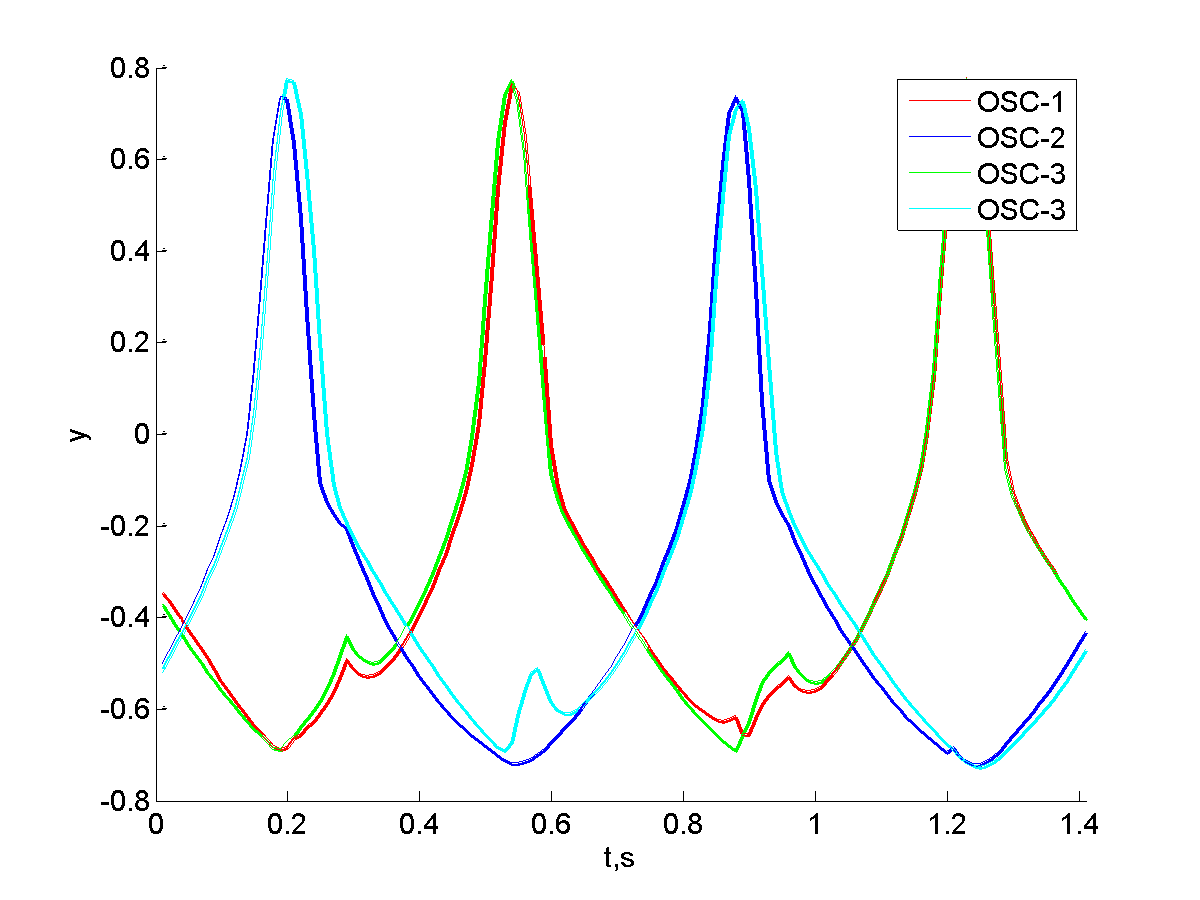
\includegraphics[scale=0.375]{cpg_time80.png}}
				\caption{CPG output state, $y_{2}$, over two gait cycles.}
				\label{fig::cpg_phase80}
			\end{figure}
			\begin{figure}[h!]
				\centering
				\fbox{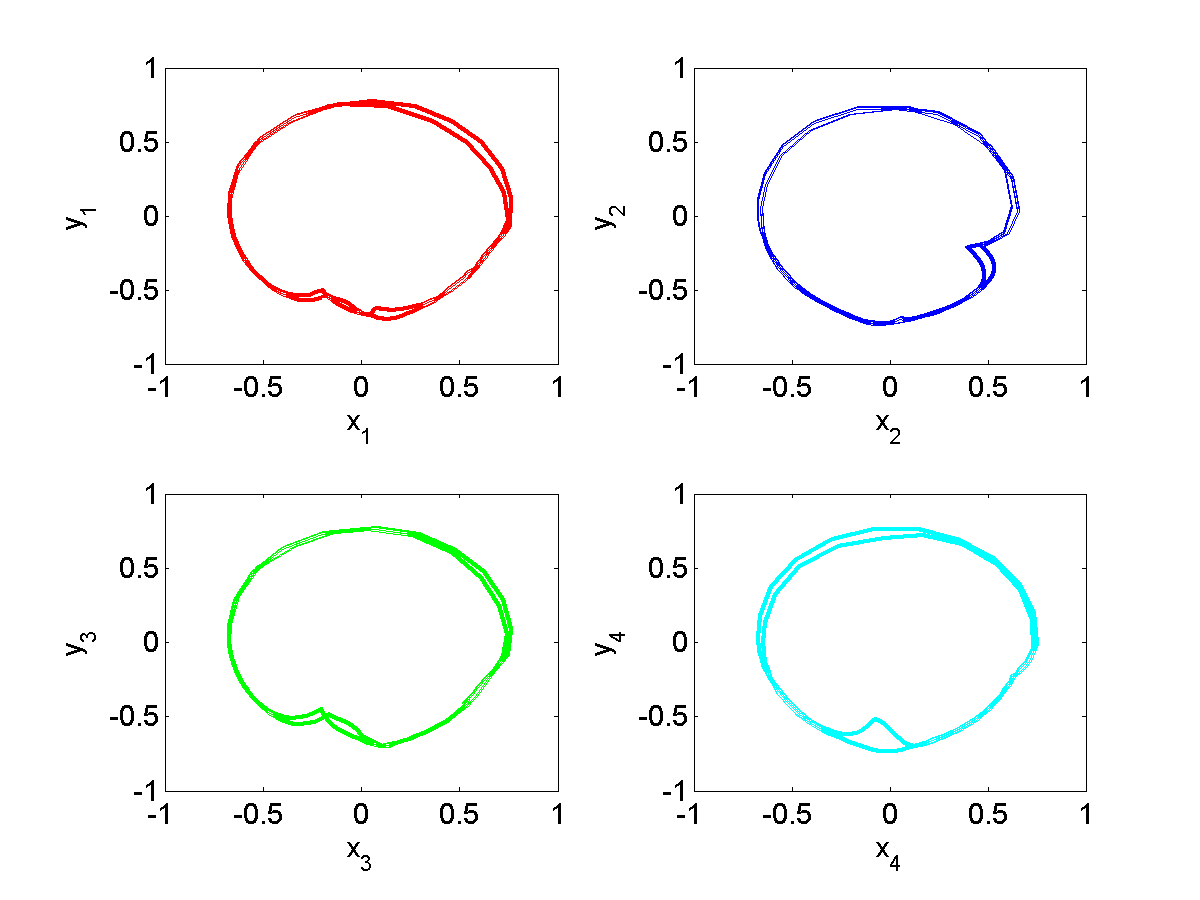
\includegraphics[scale=0.375]{cpg_phase80.png}}
				\caption{CPG state phase portrait over two gait cycles; depicts the effects of feedback-modulation on the CPG's limit cycles.}
				\label{fig::cpg_phase80}
			\end{figure}
			%%%%%%%%%%%%%%%%%%%%%%%%%%%%%%%%%%%%%%%%%%%%%%%%%%%%%%%%%%%%%%%%%%%%%%%%%%



	\section{Foot Placement Control}


		A foot placement controller has been implemented which utilizes CPG outputs (defined in equation \ref{eq:CPGMain}) in concert with a virtual-force controller. This controller is designed such that each foothold of the robot tracks the foot positions of a virtual robot generated through a model reference. The virtual robot is described by the foot positions, $\tilde{p}_{i,e}$, a virtual reference configuration corresponding to the position, $\tilde{p}_{c}$, and orientation, $\tilde{\theta}_{c}$, of the main body in $O_{0}$. The robot follows the foot placement of the virtual robot to achieve a commanded ground velocity $v_{c} \InRe{3} $; and turning velocity $\omega_{c} \InRe{}$. Each virtual point is updated by:
		\begin{eqnarray}
			\dot{\tilde{\theta}}_{c}	& = & \omega_{c} 	\nonumber\\
			\dot{\tilde{p}}_{c}			& = & v_{c}			\nonumber\\
			\dot{\tilde{p}}_{i,e} 		& = & v_{c} + \Skew{\omega_{c}\vec{h}_P} \tilde{R}_{P} \wrap{\tilde{p}_{i,e}-\tilde{p}_{c} } 
			\label{eq::virtual_foothold_control}
		\end{eqnarray}
		where $\vec{h}_P$ is a unit vector that is orthogonal and pointed outward from the surface beneath the robot and 
		$\Skew{\omega_{c}\vec{h}_P}\text{ }\in \Real^{3\times3}$ forms a skew-symmetric matrix from the vector argument $\omega_{c}\vec{h}_P$. The virtual foothold dynamics progress the target footholds at a commanded translational (forward) and rotational velocity, $v_{c}$ and $\omega_{c}$, respectively. The robot follows the virtual model at nearly the same velocities with minimal lag so long as system bandwidth is not exceeded. Using this virtual-foothold method is convenient as it allows for foot-placement planning to be independent of foot-trajectory planning. For example, terrain adaptation can be incorporated by modifying the location of virtual foot positions such that they conform to an upcoming surface. The robot's gait will then track these adaptations without any explicit modification of foot trajectories. In the event of contact with unperceived terrain, virtual-foothold positions will reset with respect to the position of the contact.

			\begin{figure}[h!]
				\centering
				\fbox{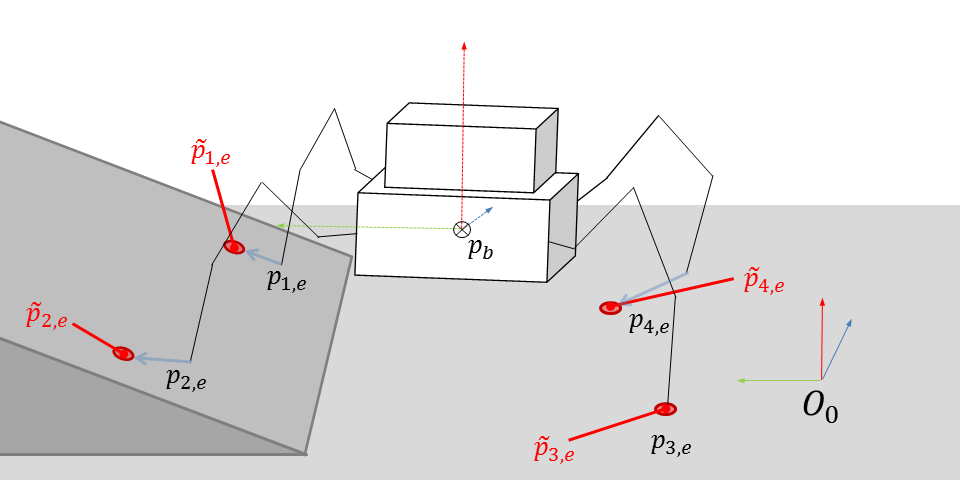
\includegraphics[width=0.75\textwidth]{virtual_foothold.png}}
				\caption{ Virtual foothold representaion. Blue arrows represent an attractive ``force" between the feet and their corresponding virtual foothold.}
				\label{fig::virtial_foothold}
			\end{figure}

		The full foothold controller represented by $\dot{p}_{i,e} = \dot{\tilde{p}}_{i,e}^{v} + \dot{\tilde{p}}_{i}^{y}, \SSep i = 1,...,4$ , is a composite of a foot-repositioning and step-height controller which are formulated in terms of the dynamics of the signals $\dot{\tilde{p}}_{i,e}^{v}$ and $\dot{\tilde{p}}_{i}^{y}$, respectively. Each foot is treated as a point mass attracted to their corresponding virtual foothold by an over-damped mass-attractor system. $\dot{\tilde{p}}_{i,e}^{v}$ is defined by
			\begin{equation}
				\label{eq::FootControl}
				\dot{\tilde{p}}_{i,e}^{v} 		= \frac{1}{m_{i}} \int^t{{P}_{\vec{h}_{i}} \wrap{ F_{s,i}  -b_{c} \dot{p}_{i,e} + F_{\epsilon,i} } d\tau}
			\end{equation}
		where
			\begin{eqnarray*}
				F_{s,i} 			& = & k_{c}  \mu_{i} \wrap{ \tilde{p}_{i} - {p}_{i,e} } \Unit{y_{2,i}}		\nonumber\\
				F_{\epsilon,i}		& = & a_{\epsilon}\dot{\epsilon}_{\theta} \Unit{y_{2,i}}						\nonumber
			\end{eqnarray*}
	 	with $k_{c},b_{c},a_{\epsilon},m_{i} \InRe{}$.
		$k_{c}$ and $b_{c}$ represent  attraction and viscous damping constants for the virtual force system. ${P}_{\vec{h}_{i}}(*)$ projects the sum of  forces, $(*)$, onto the surface beneath the \Ith foot orthogonal to $\vec{h}_{i}$. $\Unit{y_{2,i}}$ is a standard unit step function. The force $F_{\epsilon,i}$ is a compensatory force to adjust for the inertial disturbance,  $\dot{\epsilon}_{\theta}$. For instance, if the robot was pushed from the side of its body, this force would induce a side stepping motion in attempt to compensate for the disturbance. Because of $\Unit{y_{2,i}}$, $F_{s,i}$ and $F_{\epsilon,i}$ are nonzero only when $y_{2,i}$ is positive.

		The controller component $\dot{\tilde{p}}_{i,e}^{y}$ is defined from the CPG output signal $\dot{y}_{2,i}$. The height of each step is made proportional to the magnitude of desired platform velocity.
		\begin{equation}
			\dot{\tilde{p}}_{i,e}^{y} 	= \wrap{ \norm{v_{c}} a_{v} \dot{y}_{2,i}} \vec{h}_{i} 	\SSep ; \SSep a_{v}  \InRe{}.
			\label{eq::FootControl}
		\end{equation}
		Scaling step height relative to $v_c$ has been seen in experimental studies to be more effective than using a fixed step-height for all gait configurations. %In future work, step height will be modified on the basis of terrain observations.




	\section{ZMP Based Trunk-Placement Control}

		A  modified Zero-Moment-Point (ZMP) based controller is utilized in positioning BlueFoot's body during gaiting. In this context, the ZMP of the system is a set of state values for which the net-torque exerted upon the system, about the COG, is zero \cite{Kajita2003},\cite{Katie2009}. Unlike \cite{Takanishi1989,Kurazume2003}, which address ZMP-based control by considering the robot's body as point-mass with massless limbs, this method takes into account the torque contribution of each non-supporting leg. Each leg in flight is considered as a series of point masses whose locations are computed using joint position feedback and trunk orientation estimates, in concert with robot's forward kinematic model.
		
		The ZMP approach is used to first calculate static ZMP configurations ( \IE $\ddot{p}_{COG}\approx0$) at each time instance. The distance between the robot's COG and associated ZMP is incrementally minimized on-line by treating the ZMP as a  mass-attractor and ``pulling" a reference body position, ${p}_{b}^{r}$, towards the ZMP point at each update. This differs from approaches similar to \cite{Kurazume2003} because these routines feature off-line, trunk trajectory design which aim to minimize deviations between the robot's COG and ZMP by creating an appropriate limit-cycle motion for the robot's trunk. These approaches typically utilize simplified, linearized models of the actual system about marginally-stable equilibrium points. To realize an adjustment of the robot's COG, towards the ZMP, BlueFoot's trunk position is modified during the execution of a gait. The trunk is controlled (and not individual feet) as it contributes most of the system's total mass and, thus, has the greatest influence over the location of the platform's COG. Restricting adjustments to the trunks translational states allow pre-planned foot trajectories to remain unmodified by the ZMP-control module during gait execution, thus decoupling foot-placement and body-placement control.

		To incrementally compute the static ZMP of the platform, a measure of net-moment on the body of the platform must be known. The net-moment due to gravitational forces, $\tau_{net}$, is approximated using the locations of each link and joints as point-mass loads. Hence, $\tau_{net}$ is calculated as follows:
			\begin{equation}
				\tau_{net} 	= \vec{g} m_{P}  \wrap{\bar{p}_{b}-\hat{p}_{COG} }	+ \tau_{legs}
				\label{eq::NetMoment}
			\end{equation}
		where
			\begin{eqnarray*}
					\tau_{legs}		& = & \Sum{i}{1}{4} (1-\mu_{i})  \Sum{i}{1}{4} \vec{g} \times  \wrap{ m_{i,j}^{J} d_{i,j}^{J} + m_{i,j}^{L} d_{i,j}^{L} }	\nonumber \\
					d_{i,j}^{J} 	& = & {{p}_{i,j}-\hat{p}_{COG}.} \nonumber \\														
					d_{i,j}^{L} 	& = &
					\begin{cases}
					{ 0.5  \wrap{{p}_{i,j+1}-{p}_{i,j}} + {p}_{i,j} - \hat{p}_{COG}} 	& \If j < 4 \\
					{ 0.5  \wrap{{p}_{i,e}-{p}_{i,j}} + {p}_{i,j} - \hat{p}_{COG}} 		& \If j = 4
					\end{cases} \nonumber
				\label{eq::Levers}
			\end{eqnarray*}
		with $m_{P}$, $m_{i,j}^{J}$ and $m_{i,j}^{L}$ represent the mass of the main body; the mass of each joint; and the mass of each link, respectively. $\mu_{i}$ is included in the above formulation such that only stepping legs contribute to  $\tau_{legs}$. The estimated center of gravity, $\hat{p}_{COG}$, is generated as follows:
			\begin{eqnarray*}
				\hat{p}_{COG} 	& = & \frac{1}{m_{T}}\wrap{ m_{b}p_{b} + \sum_{i=1}^{4} \wrap{m_{i,e}{p}_{i,e} + \sum_{j=1}^{4} \wrap{  m_{i,j}^{J}{p}_{i,j} +  m_{i,j}^{L}{p}_{i,j}^{L} } }} 	\nonumber \\
				{p}_{i,j}^{L} 	& = & 
					\begin{cases}
					{ 0.5  \wrap{{p}_{i,j+1}-{p}_{i,j}} + {p}_{i,j} } 	& \If j < 4 \\
					{ 0.5  \wrap{{p}_{i,e}-{p}_{i,j}} + {p}_{i,j} } 		& \If j = 4
					\end{cases} \nonumber
				\label{eq::cog_estimate}
			\end{eqnarray*}
		where
			\begin{equation}
				m_{T} = m_{b} + \sum_{i=1}^{4} \wrap{m_{i,e} + \sum_{j=1}^{4} \wrap{  m_{i,j}^{J} +  m_{i,j}^{L} } }
			\end{equation}

		Setting $\tau_{net}=0$, (\ref{eq::net_moment}) is manipulated to a derived solution for the ZMP as follows:
			\begin{equation}
				{p}_{ZMP} = R_{z_P} \wrap{\frac{\pi}{2}}  \wrap{ \norm{g}/m_{P}} \tau_{legs} + \hat{p}_{COG}.
				\label{eq::ZMPFromMoment}
			\end{equation}

		Using ${p}_{ZMP}$, the platform's posture is then updated using a virtual-force controller. Moreover, ${p}_{b}$ is to be controlled through  ${p}_{b}^{r}$ such that it is smoothly attracted to ${p}_{ZMP}$. The controller is given by
			\begin{equation}
				\dot{p}_{b}^{r} 	= \frac{1}{m_{P}} \int^{t} {P}_{\vec{h}_{i}} \wrap{K_{ZMP}	( {p}_{ZMP} - {p}_{b} )  
				+ F_{r} } d\alpha
				\label{eq::ZMPController}
			\end{equation}	
		where
			\begin{eqnarray*}
				F_{r} 	& = &  \Sum{i}{1}{4} \exp \wrap{k_{l} \wrap{r_{min} -  \norm{r_{i}}}} + \exp \wrap{k_{l} \wrap{ \norm{r_{i}} - r_{max}}} \nonumber \\
				r_{i}	& = & {p}_{i,e}- {p}_{b} \nonumber
			\end{eqnarray*}
%%
		and $K_{ZMP}, K_{c}, K_{\epsilon}, k_{l} > 0$ and $\dot{p}_{b}^{r}$ is the reference body velocity. $F_{r}$ is a boundary force added to ensure that the workspace of each manipulator, defined by the radii $r_{min}$ and $r_{max}$, is not exceeded when the body is repositioned. $k_{l}$ is picked to be adequately large such that this force is nearly zero when the body and foot positions comply with the local workspace of each leg, and large when the workspace is nearly compromised, forcing the placement of the body to comply with each leg workspace.





	\section{Trunk Leveling NARX-Network Learning Approach}

		Disturbance rejection from the trunk sub-system of a legged platform has practical significance when carrying a payload (such as cameras, optical systems, armaments, etc.) rigidly fixed to their main body. Disturbances are imparted upon the trunk during gaiting in two main ways: 1) instantaneous changes in force distribution when feet make and break contact with the ground, and 2) under-actuation that occurs during certain dynamic gaits. During dynamic gaits, such as trot gaits, the state of contact between the feet and the ground is changed often so as to prevent the walking robot from tipping past a recoverable configuration. Additionally, these gaits feature the utilization of two or fewer legs to support the trunk at any given time, causing the 
		system to enter an under-actuated state where the body is free to rock about the planted feet, as shown in Figure \ref{fig::quadruped_walking}.

			\begin{figure}[h!]
			\centering
				\fbox{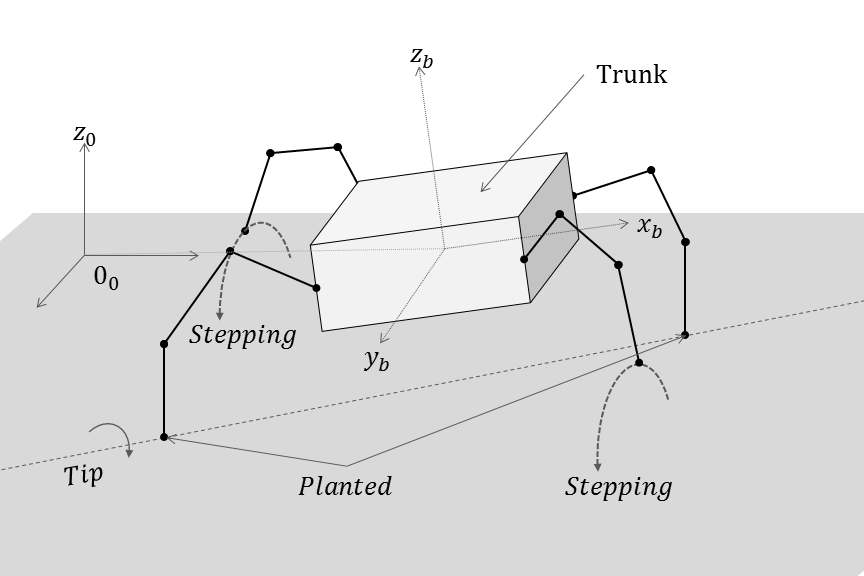
\includegraphics[width=0.75\textwidth]{tipping_robot.png}}
				\caption{ Quadruped tipping about planted feet. }
				\label{fig::quadruped_walking}
			\end{figure}

		To achieve disturbance rejection on the trunk orientation and to attain a fixed orientation, experimentation has been performed using a control methodology which utilizes a Nonlinear Autoregressive Neural Network with Exogenous inputs (NARX-NN) as part of an active compensation mechanism. The network is used to estimate the system dynamics and, further, predict periodic disturbances in an on-line fashion. The compensator is utilized to modify referential joint trajectories by way of a weighted sum between the original joint trajectories generated by the gaiting mechanism and a reference correction signal generated by the compensator.

		\subsection{NARX-Neural Network}

			%%% MPC Controller %%%
			A NARX-NN architecture is used in this controller because of  its known effectiveness in approximating nonlinear difference systems and making multivariate time-series predictions \cite{Tsungnan1996,ChenBillings1990,Hihi1996,Billings2013}. Moreover, the NARX-NNs is a natural fit for a problem of this nature where the dynamics being considered are both periodic and of a high enough complexity where a nonlinear approximation method is warranted. The parallel NARX-NN model, shown in Figure \ref{fig::narx_net}, is comprised of a feed-forward neural network whose input layer accepts a series of time-delayed system state values and network-output histories. The NARX-NN is trained to predict system states in the next time-instant from these inputs. Conveniently, NARX-NN training can be performed using standard BP because recurrence occurs between network inp
uts and outputs, and not within the hidden layers \cite{Nelles2001}.

			The NARX-NN is trained to capture the effects of forces and moments and dynamical couplings that act on the trunk
			so that an appropriate torque input to the joints is computed to reduce such effects on trunk orientation while performing the gate. This is achieved by considering the inverse dynamics corresponding to joint motion.

			Disturbances imparted upon the trunk during gaiting manifest in the term $\Phi$, largely as a result of variations in $f_{ext}$ and associated effects due to dynamical coupling. Because of this, the NARX-NN will learn an estimate for $\Phi$, denoted $\hat{\Phi}$. The network is trained on-line using the standard incremental back-propagation (BP) algorithm with an adapted learning rate, $\gamma^{lr}$ and momentum term, $\mu$ \cite{Rumelhart1988,Rumelhart1995}. This error BP algorithm is a gradient-descent based method used to train a feed-foward nueral network with $n$-layers and layer-connection matrices $\setwrap{W^{1},W^{2},...,W^{n-1}} \in \emph{W}$. The BP algorithm, as used in this control approach, is summarized in matrix-vector form in (adapted from \cite{Rojas1996ch7}) as follows: 

			\begin{equation}
				\Delta W^{i} =
					-\gamma^{lr} \wrap{ \frac{ \partial o^{i} }{\partial {W^{i} } }  o^{i-1} }^{T}  + \mu \Delta W^{i} = 
					-\gamma^{lr} \delta^{i} \wrap{o^{i-1}}^{T}  + \mu \Delta W^{i}
				\label{eq::bp_weight_update}
			\end{equation} 
			%
			where
			%
			\begin{equation*}
				\delta^{i} = \wrap{ \nabla_{y} \sigma^{i}\wrap{y^{i}} } e^{i}
				\label{eq::bp_error}
			\end{equation*}
			\begin{equation*}
				y^{i} = W^{i} o^{i-1}
				\label{eq::bp_error}
			\end{equation*}
			\begin{equation*}
				e^{i} =  \wrap{ W^{i} }^{T} \delta^{i+1} \hspace{2mm} \forall \hspace{2mm} i\neq n,
			\end{equation*}
%%
			$\gamma^{lr} \in [0,1]$, the learning and  $\mu \in [0,1]$, the learning momentum; $W^{i} \in \Re^{N_{O}^{i}\times N_{I}^{i}}$, which represents the weighting matrix between the \Ith layer (of size $N_{I}^{i}$ nodes) and $(i+1)^{th}$ layer (of size $N_{O}^{i}=N_{I}^{i-1}$); $\Delta W^{i}$, which represents the corresponding weight update to $W^{i}$; and $e^{i}$ is the ouput error for each \Ith layer. For the output ($n^{th}$) layer, $e^{n}$ is equal to the difference between the network output and the network output target, which will be defined later. For all other layers, $e^{i}$ represents a \emph{back-propogated} error. from the $(i+1)^{th}$ layer.


%%
			$\sigma^{i}(y^{i})$ is a layer-wise activation function which outputs a vector of scalar activation outputs, $\sigma_{j}^{i}(y_{j}^{i}) $ for each \Jth, weighted input, $y_{j}^{i}$, defined as follows:
			\begin{equation*}
				\setwrap{ \sigma^{i}(y^{i}) = \sbrack{ \sigma_{1}^{i}(y_{1}^{i}),...,\sigma_{N_{I}^{i}}^{i}(y_{N_{I}^{i}}^{i}) }^{T} \hspace{2mm} : \hspace{2mm} \Re^{N_{I}^{i}} \rightarrow \Re^{N_{I}^{i}}}
			\end{equation*}
For the control approach being described, each $\sigma_{j}^{i}(y_{j}^{i}) \equiv \tanh(y_{j}^{i}) \in [-1,1]$. Hence the gradient $\nabla_{y} \sigma^{i}(y^{i})$ is defined as follows: 
			\begin{equation}
				\nabla_{y} \sigma^{i}(y^{i})  = \text{diag}\wrap{\sigma^{i}(y^{i})} \wrap{\vec{1}_{N_{I}^{i}\times1} - \sigma^{i}\wrap{y^{i} } }
				\label{eq::bp_sigmoid_deriv}
			\end{equation} 
			given the derivative properties of the $\tanh\wrap{*}$ function.
			
The success of this learning mechanism, as it applies to the presented controller, is predicated on the periodicity of the system dynamics during gaiting. Like any BP-trained neural network, repetition of similar input and output sets is paramount for successful network training and, by extension, prediction accuracy. It is assumed that this specification can be met given the inherently cyclic nature of the dynamics being estimated during gaited locomotion. 
			%%%
			%%%
				\begin{figure}[t!]
					\centering
					\fbox{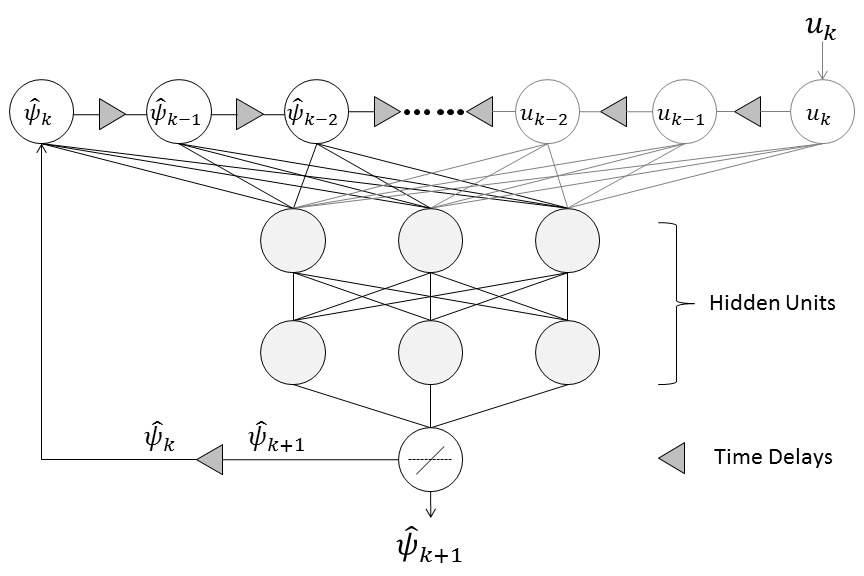
\includegraphics[width=0.75\textwidth]{narx_network_diagram.png}}
					\caption{Parallel NARX-network model with a linear output layer.}
					\label{fig::narx_net}
				\end{figure}
			%%%
			%%%
			Using the NARX-NN, the dynamical estimate $\hat{\Phi}_{k}$ is generated as a prediction of the sampled system dynamics, $\hat{\psi}_{k+1}$. The relationship between $\hat{\Phi}_{k}$ and the network prediction $\hat{\psi}_{k+1}$will be made clear in the description of the network training signal given in \ref{eq::training_signal}. The general input-output relationship of the NARX-NN predictor, $\emph{N}$, is described as follows:
			%%%
			%%%
				\begin{eqnarray}
					\hat{\psi}_{k+1}	&=& \emph{N}(\hat{\Psi}_{k}^{N},{U}_{k}^{N}) \nonumber\\
					\hat{\Psi}_{k}^{N}	&=& [\hat{\psi}_{k},\hat{\psi}_{k-1},...,\hat{\psi}_{k-N+1}]  \nonumber\\
					{U}_{k}^{N}		&=& [u_{k}   ,u_{k-1}   ,...,u_{k-N+1}   ]
					\label{eq::narx_model}
				\end{eqnarray}
			%%%
			%%%
			where ${U}_{k}^{N}$  and $\hat{\Psi}_{k}^{N}$ are collections of $N$ most recent samples of the network inputs, $u_{k}$, and the network output, $\hat{\psi}_{k}$, respectively. The NARX-NN input, $u_{k}$, represents a tuple $u_{k} = (z_{1,k}, z_{2,k}, f_{ext,k})$ whose components are the arguments of $\Phi$ at time instant $k$. 



		\subsection{NARX-NN Training Regimen}
			
			The  NARX-NN training signal is formulated to estimate $\Phi_{k}$ from the system dynamics. By \ref{eq::sampled_dynamics}, it can be seen that $\Phi_{k}$ can be estimated if ${z}_{2,k+1}$ can be predicted. We consider the following target network prediction output, $\psi_{k+1}$,  defined by:
				\vspace{-2mm}
				\begin{equation}
					\psi_{k+1} = \tau_{k} - \hat{M}_{1,k}({z}_{2,k+1} - {z}_{2,k})\Delta_{s}^{-1} = \Phi_{k} - {e}_{2,k}^{\Delta_{s}} \text{ .}
					\label{eq::training_signal}
				\end{equation}
			%%
			%%
			This training signal formulation assumes that $\hat{M}_{1,k}$ represents $M_{1,k}$ exactly, which is likely not the case given the system's complexity. In the absence of a well-modeled $\hat{M}_{1,k}$, a constant symmetric $\hat{M}_{nom}$ will be picked such that $\hat{M}_{1,k} = \hat{M}_{nom} \forall k$. $\hat{M}_{nom}$ has the following structure:
				\begin{equation}
					\hat{M}_{nom} = \left[
						\begin{array}{cc}
						\hat{M}_{bb}	&	 \hat{M}_{bq}\\
						\hat{M}_{qb}	&	 \hat{M}_{qq}
						\end{array}
					\right]
				\end{equation}
			where 	$\hat{M}_{bb}\RealMat{6}{6}$, 
					$\hat{M}_{bq}=\hat{M}_{qb}^{T} \RealMat{6}{16}$, and  
					$\hat{M}_{qq}\RealMat{16}{16}$. 
			It is particularly important that $\hat{M}_{bq}\neq0$ to reflect some degree of coupling between the joint states $q$ and the trunk states ${p}_{b}$ and $\theta_{b}$. In general, if $\hat{M}_{nom}$ should be selected to reflect the \emph{average} system mass matrix over the range of configurations, $z_{1}$, seen during gaiting. This approximation has shown to be adequate from our results, and depends on the assumption that changes in $\hat{M}_{1,k}$ are small  over the subset of state $z_{1}$ experiences during a periodic gaiting sequence. Future improvements of this controller involve the formulation of a separate estimator for $M(z_{1})$, or a control/learning scheme with no direct dependence on $M(z_{1})$.

			Since $\hat{\psi}_{k+1}$ is non-causal, training is performed one time-step after a prediction is made using the input-output pair $\hat{\psi}_{k}$ and \{${\Psi}_{k-1}^{N}$, ${U}_{k-1}^{N}$\}. Note that $\hat{\psi}_{k}$ can calculated directly using \ref{eq::training_signal} where all component signals are time-delayed by one time-step. Training can then be described by:
				\begin{equation}
					\psi_{k} \xrightarrow{BP(\gamma^{lr})} \emph{N}({\Psi}_{k-1}^{N},{U}_{k-1}^{N})
					\label{eq::training}
				\end{equation}
			where $\gamma^{lr} _{min} < \gamma^{lr} < \gamma^{lr} _{max}$ is a learning rate adapted using a \emph{bold-driver} update routine. Bold-driver learning-rate adaptation is a  heuristic method for speeding up the rate of convergence of back-propagation training regimes \cite{Battiti1992,Magoulas1999}. This $\gamma^{lr}$ update law is parameterized by $\beta \in (0,1)$ and $\zeta \in (0,1)$ which are selected to specify the amount by which $\gamma^{lr}$ increases or decreases per update, and $\gamma^{lr} _{min}$ and $\gamma^{lr} _{max}$ which are used to saturate $\gamma^{lr}$.  The bold-driver scheme utilizes the current and previous mean-squared network output error values ($MSE_{k}$ and $MSE_{k-1}$, respectively) to adjust $\gamma^{lr}$ as follows:
				\begin{equation}
				    \gamma^{lr} \leftarrow 
					\begin{cases}
				    \gamma^{lr} (1- \beta) 		& \text{if } MSE_{k} > MSE_{k-1}\\
				    \gamma^{lr} (1+\zeta \beta),& \text{otherwise}.
					\end{cases}
				\end{equation}
			Since network training is being performed on-line as an incremental routine, the effective mean-squared NARX-NN  output error is low-passed by a factor $\lambda \in (0,1)$. This update technique has been selected to ensure that outliers presented during training do not affect network learning updates as significantly as ``nominal" training pairs. Network output error, $e_{\emph{N},k}$, and its associated MSE values are calculated after each prediction by:
				\begin{eqnarray}
					e_{\emph{N},k} 	&=& \hat{\psi}_{k} - \psi_{k} \nonumber\\
					MSE_{k} 		&\leftarrow& \lambda \|e_{\emph{N},k}\|_{2}^{2} + MSE_{k-1}(1-\lambda).
				\end{eqnarray}


		\subsection{Compensator Output}

			The control scheme is first presented with respect to the servo input torques, $\tau_{q,k}$, and formulated to achieve a level trunk characterized by $\theta_{b}=0$, $\dot{\theta}_{b}= 0$. To formulate this controller, the dynamical sub-system which corresponds to the un-actuated trunk orientation states is isolated by:
				\begin{equation}
					\ddot{\theta}_{b} 	= \Gamma_{1} M^{-1}(z_{1})( \Gamma_{2}\tau_{q}	 + \Phi)
					\label{eq::sub_dynamics}
				\end{equation}
			where 
				\begin{eqnarray*}
					\Gamma_{1} &=& [0_{3\times3},I_{3\times3},0_{3\times16}] \nonumber\\
					\Gamma_{2} &=& [0_{16\times6},I_{16\times16}]^{T}	
				\end{eqnarray*}
			and $\Gamma_{2}\tau_{q}$ is equivalent to the original system input, $\tau$. In order to enforce a level platform with zero angular velocity, we seek a $\tau_{q}$ which emulates the proportional-derivative (P.D.) control law:
				\begin{equation}
				 	\ddot{\theta}_{b} = - K_{b}{\theta}_{b} - K_{d}\dot{\theta}_{b}
				\end{equation}
			where $K_{b}$ and $K_{d}$ are constant gain matrices. Using this P.D. law and \ref{eq::sub_dynamics}, we propose a least-squares solution for $\tau_{q}$ by:
				\begin{equation}
					\tau_{q} \approx -\left[\Gamma_{1} M^{-1}(z_{1}) \Gamma_{2}\right]^{\dagger}\Gamma_{1} M^{-1}(z_{1})(\Phi + K_{b}{\theta}_{b} + K_{d}\dot{\theta}_{b} )
					\label{eq::psuedo_torque}
				\end{equation}
			where $\left[*\right]^{\dagger}$ denotes the Penrose-Moore pseudo-inverse of $[*]$.
			%%
			Replacing all dynamical terms with their associated discrete-time equivalents, and $\Phi$ by the NARX-NN output $\hat{\Phi}_{k}=\hat{\psi}_{k+1}$, we apply (\ref{eq::psuedo_torque}) to arrive at the following required joint torque estimate:
				\begin{equation}
					\hat{\tau}_{q,k} =  -\left[\Gamma_{1} \hat{M}^{-1}_{1,k} \Gamma_{2}\right]^{\dagger} \Gamma_{1}\hat{M}^{-1}_{1,k}( \hat{\psi}_{k+1} + K_{b}{\theta}_{b,k} + K_{d}\dot{\theta}_{b,k} )
					\label{eq::psuedo_torque_k}
				\end{equation}
			where ${\theta}_{b,k}$ and $\dot{\theta}_{b,k}$ are samples of angular trunk position and rate, respectively.


			Using the joint controller dynamics presented in \ref{eq::joint_dynamics} and the estimate $\hat{\tau}_{q,k}$, we can formulate a reference-trajectory correction  which is used to alter the joint reference positions, ${q}_{k}^{r}$. Moreover, the corrected reference position, ${q}_{1,k}^{r,*}$ is generated such that the estimated output torque $\hat{\tau}_{q,k}$ is attained by each joint controller. This joint-reference compensator output is defined using 
			\ref{eq::psuedo_torque_k} as follows:
				\begin{equation}
				 	{q}_{1,k}^{r,*} 	= k_{s}^{-1}  \left(  \hat{\tau}_{q,k}  \right) +  {q}_{1,k}.
					\label{eq::correction_equation}
				\end{equation}
			The correction signal,  ${q}_{k}^{r,*}$, is combined with the original gaiting trajectory signal, ${q}_{k}^{r}$, as a weighted sum to form a compensated joint control reference signal, $\tilde{q}_{k}^{r}$, defined by:
				\begin{equation}
				 	\tilde{q}_{k}^{r} 	\leftarrow (1-\alpha) {q}_{k}^{r} + \alpha ( {q}_{k}^{r,*} )
					\label{eq::correction_application}
				\end{equation}
			where  $\alpha \in (0,1)$ is a uniform mixing parameter. The parameter $\alpha$ must be tuned with respect to the stability margins of the gait being compensated. The resultant $\tilde{q}_{k}^{r}$ is then applied  to each joint controller in place of the original reference signal,  ${q}_{k}^{r}$,  generated by the gait controller. Selection of the parameter $\alpha$ is crucial for achieving good performance. 

				\begin{figure}[h!]
					\centering
					\fbox{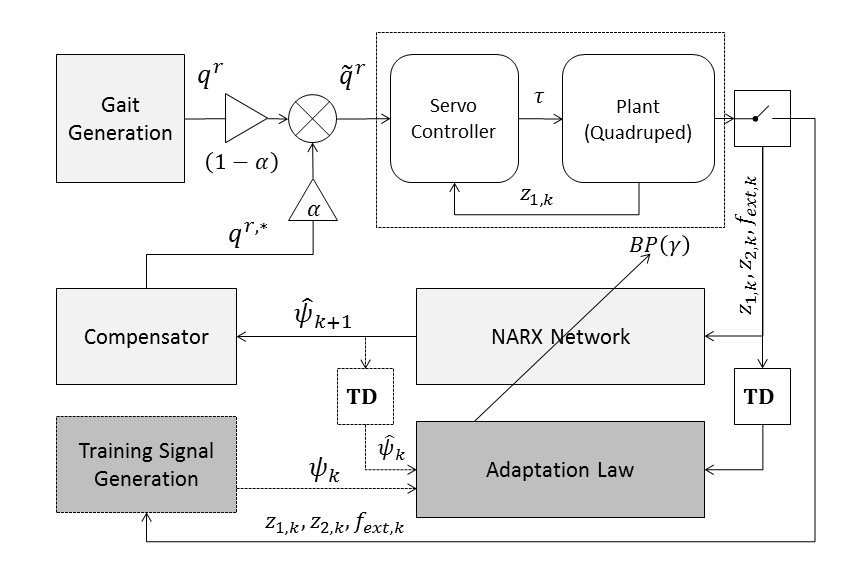
\includegraphics[width=0.75\textwidth]{controller_diagram.png}}
					\caption{Full system diagram with NARX-NN compensator mechanism.}
					\label{fig::sys_diagram}
				\end{figure}

		\subsection{NARX-NN Compensator Results}
			The NARX-NN compensator has been tested, exclusively, in simulation and has been applied to applied to the quadruped as it executes a stable CPG-driven trot gait depicted in Figure~\ref{fig::quadruped_walking}. In these trials, gaiting frequency is adjusted accordingly to achieve particular forward speeds. NARX-NN parameters are fixed for all trials with learning-rate  parameters set to $\beta=0.0001$, $\zeta=0.0005$ and $\lambda = 0.01$. The NARX-Network is configured with two hidden layers containing 50 neurons each. Each input and hidden-layer neuron is modeled using a symmetric sigmoid activation function. Output layer neurons are modeled using linear activation functions to  avoid output-scaling saturation issues. Figure~\ref{fig::fast} exemplifies the convergence of the NARX-NN prediction error when the platform executes a gait at  100~$\frac{mm}{s}$ with $\alpha = 0.35$.
%
			\begin{figure}[h!]
				\centering
				%\begin{subfigure}{0.475\textwidth}
					%\centering
					%\SetImage{\ImageWidthRatioSub}{aux_V_80mms_nN_50_nL_2_pos.png}
					%\caption{ }
				%\end{subfigure}
				%\begin{subfigure}{0.475\textwidth}
					%\centering
					%\SetImage{\ImageWidthRatioSub}{aux_V_100mms_nN_50_nL_2_pos.png}
					%\caption{ } 
				%\end{subfigure}
				%\begin{subfigure}{0.475\textwidth}
					%\centering
					%\SetImage{\ImageWidthRatioSub}{aux_V_100mms_nN_50_nL_2_nns.png}
					%\caption{ } 
				%\end{subfigure}
				\caption{ 
					\textbf{a)} Trunk orientation during 80 $\frac{mm}{s}$ gait with mixing  parameter set to $\alpha = 0.35$; \textbf{b)} Trunk orientation during 100 $\frac{mm}{s}$ gait with mixing parameter set to $\alpha = 0.35$; \textbf{c)} NARX Network MSE convergence for trial shown in \textbf{(b)}.
				}
				\label{fig::fast}
				%\PostImageCloseSpace
			\end{figure}

			All simulated trials are performed over a period of 60 seconds each. During the first 10 seconds of each simulation, the robot moves from sitting position to a standing position and initiates walking. During each simulation period, the NARX-NN compensator is activated (not training)  and deactivated (training)  every 10 seconds. Figure~\ref{fig::alpha_tests} depicts initial set of simulation results showing the effect of varying  the mixing parameter $\alpha\in\{0.125, 0.25, 0.35\}$. For all such trials, the robot performs a trot-gait which achieves a forward speed of 60 $\frac{mm}{s}$. We expect that as $\alpha$ increases, the compensator will have greater authority over trunk stabilization. From these results, we observe that for all $\alpha$, disturbance magnitude is decreased to some extent. However, for smaller $\alpha$, the compensator is less effectual due to the fact that it has less authority over joint reference signals.  From the results in Figure~\ref{fig::alpha_tests} \textbf{c)}, we see that the compensator improves pitch stability by more than roughly 50\% and roll stability by more than 60\%. Figure~\ref{fig::fast} shows the compensator's performance at higher gaiting speeds of 80 $\frac{mm}{s}$ and 100 $\frac{mm}{s}$. Here the controller improves both pitch and roll by nearly 50\% and 40\% of the  uncompensated signal magnitude, respectively.